\section{Experiments for Proposal 2}\label{section:experiment_part_2}

\textit{Multi-instance Learning}\footnote{Also called \textit{Multiple-instance} Learning} is a technique (the name was first coined by \cite{dietterich_etal_1997}), whereby a an  instance in a traditional supervised learning problem is split into multiple so-called \textit{bags}.

In other words, each individual sample in a dataset is represented not by a single feature vector but by a set thereof. For example, images may be represented as a bag of patches \citep{maron_ratan_98,andrews_etal_2003}, pharmacological drug molecules may be represented as a bag of configurations \citep{dietterich_etal_1997,andrews_etal_2003}.

\begin{figure}[H]
    \centering
    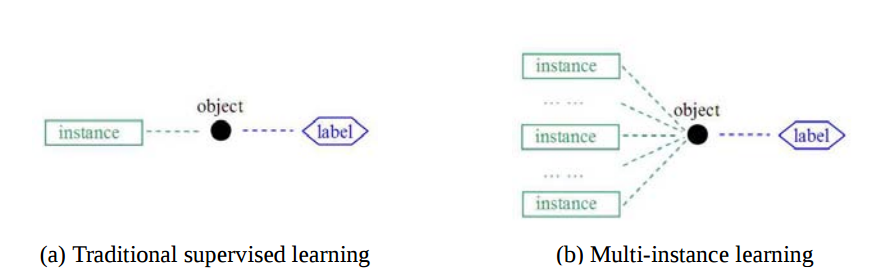
\includegraphics[width=0.8\textwidth]{chapters/05_experiments/images/miml1.png}
    \caption{Multi-instance learning works by representing a single example as multiple instances.}
    \label{fig:mimlsvm1}
\end{figure}

In 2006, \citeauthor{zhou_zhang_2006} have adapted the multi-instance learning paradigm into the multi-label setting, in the context of \textit{scene classification}. The main insight put forward by this work is that a multi-instance, multi-label (MIML) problem can be transformed into either \textbf{a)} a single-instance, multi-label task or \textbf{b)} a multi-instance, single-label task:

\begin{figure}[H]
    \centering
    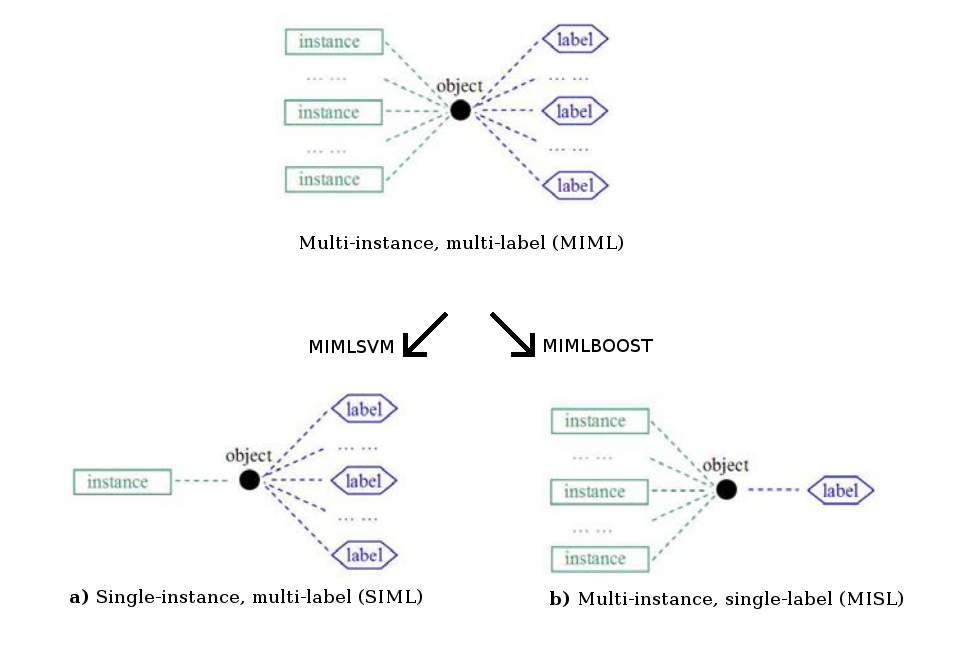
\includegraphics[width=\textwidth]{chapters/05_experiments/images/miml2.png}
    \caption{Original algorithm, devised by \cite{zhou_zhang_2006}, transforms an MIML problem into either a SIML or an MISL problem, using MIMLSVM and MIMLBOOST techniques, respectively.}
    \label{fig:mimlsvm1}
\end{figure}

In 2009, \citeauthor{shen_etal_2009} have applied multi-instance, multi-label (MIML) learning to the tag prediction problem. In particular, they have adapted the MIMLSVM algorithm from \cite{zhou_zhang_2006} to multi-label text classification.

The main idea here is that a single textual document may be split into multiple \textit{segments} via some kind of text segmentation algorithm. This makes it possible to view this problem as a multi-instance, multi-label (MIML) problem, where each segment represents one of many instances for a single document.

Each document is split into segments using a well-known text segmentation algorithm called \textit{TextTiling} (\cite{hearst_1994}). Then, these segments are vectorized into bag-of-words vectors. In order to turn the multiple segments into a single instance, the authors use \textit{k}-medoids clustering based on the Hausdorff distance (\cite{edgar_2008}). Finally, an SVM classifier\footnote{Configured so that it predicts a real-valued score for each tag instead of a binary prediction.} is applied on to the transformed dataset.\\ \\

\begin{algorithm}[H]
\LinesNotNumbered
\SetKwInOut{Input}{input}\SetKwInOut{Output}{output}
\Input{A set $D$ of text documents}
\Output{A trained SVM model to rank tags $y_d$ for every $d$ in $D$}
\BlankLine
 \textbf{Part I: Building a Single-Instance Dataset}
 
\ \ForEach{document $d$ in $D$}{
\BlankLine  
\tcp{split document into segments}\label{cmt}
$segments_d \leftarrow TextTiling(d)$    
  
  \BlankLine
  \BlankLine
  \tcp{transform each segment into a vector of features}\label{cmt} 
  $vectorizedSegments_d \leftarrow extractFeatures(segments_d)$ 
  
  \BlankLine
  \BlankLine
  \tcp{apply $k-$medoids clustering algorithm to the segments of $d$.}\label{cmt}
  \tcp{note that $features_d$ is now a single-instance vector}\label{cmt}
  \tcp{because Hausdorff Distance was used in clustering}\label{cmt}
  $features_d \leftarrow kMedoids( vectorizedSegments_d)$
  \BlankLine
  \BlankLine
  \tcp{this becomes a single row in the new $D'$ dataset}\label{cmt}
  $D'_d \leftarrow features_d$ 
 }
   \BlankLine
  \BlankLine
 \textbf{Part II: Training an SVM Classifier on $D'$}
 \caption{MIMLSVM applied to Tag Prediction \citep{shen_etal_2009} }
\ Train a $Ranked$ SVM algorithm on the transformed features in $D'$
\end{algorithm}

\hfill \break

The objective of the experiments in this section is to ascertain whether (if at all) the original results generalize to other kinds of features.

\subsection{MIMLSVM with IDF weighted Bag-of-words features}

\subsubsection{Results on dataset 1}

\subsubsection{Results on Dataset 2}

\begin{figure}[H]
    \centering
    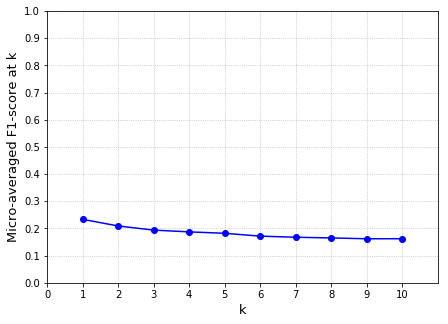
\includegraphics[width=7cm]{chapters/05_experiments/images/mimlsvm-tf-idf-movielens.png}
    \caption{MIMLSVM classifier applied on the Movielens dataset, using TF-IDF weighted bag-of-words features.}
    \label{fig:knn_lda_movielens}
\end{figure}

\subsubsection{Discussion}

\subsection{MIMLSVM with LDA Topic Probabilities as Features}

\subsubsection{Results on dataset 1}

\subsubsection{Results on Dataset 2}

\subsubsection{Discussion}

\subsection{MIMLSVM with IDF-weighted Bag-of-embeddings Features}

\subsubsection{Results on dataset 1}

\subsubsection{Results on Dataset 2}

\subsubsection{Discussion}